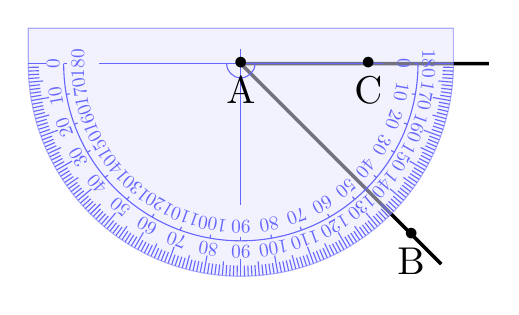
\begin{tikzpicture}[scale=.9]

\def \RotFigure {0} %rotation de toute la figure y compris textes
\begin{scope}[rotate=\RotFigure]

\def \CharSize {1.4};
\def \BulletSize {1};
\coordinate (A) at (0,0);
\coordinate (B) at (2.404,-2.404);
\coordinate (C) at (1.8,0);
\coordinate (U) at (3.5,0);
\coordinate (V) at (2.828,-2.828);

\draw[line width = 1.3pt] (U) -- (A) -- (V);
	
%début du rapporteur
    %Définition de l 'angle de rotation du rapporteur
    \def \RapRot {180} 
    %Définition du décalage du rapporteur
    \def \DecalX {0}
    \def \DecalY {0}
    %Couleur des élèments du rapporteur (sauf le remplissage)
    \def \RapColor {blue!60}

\begin{scope}[shift={(\DecalX,\DecalY)},rotate=\RapRot]
    % contours du rapporteur
    \draw[color=\RapColor, fill =blue!10, opacity=0.5] (-3,0) arc(180:0:3)--(3,-0.5)--(-3,-0.5)--cycle;	%Dont couleur de remplissage
    \draw[color=\RapColor] (-2,0)--(2,0);
    \draw[color=\RapColor] (0,-0.2)--(0,2);
    % graduation externe 1 degrés
    \foreach \a in {0,1,...,180}{\draw[color=\RapColor] (\a:3)--(\a:2.85);}
    % graduation externe 5 degrés
    \foreach \a in {0,5,...,180}{\draw[color=\RapColor] (\a:2.85)--(\a:2.8);}
    % double graduation
   \foreach \a/\b in {%
        0/-90,10/-80,20/-70,30/-60,40/-50,50/-40,%
        60/-30,70/-20,80/-10,90/0,100/10,110/20,%
        120/30,130/40,140/50,150/60,160/70,170/80,180/90%
    }{
    % graduation externe 10 degrés
    \draw[color=\RapColor] (\a:2.80)--(\a:2.75) 
    node[scale=0.7, rotate=\b+\RapRot+\RotFigure] (\a) at (\a:2.65){\a};
    % graduation interne 10 degrés
    \draw[color=\RapColor] (\a:2.5)--(\a:2.45)
	node[thin,scale=0.7, rotate=-\b+\RapRot+\RotFigure] (\a) at (180-\a:2.3){\a}; }
    % demi-cercle intérieur
    \draw[color=\RapColor](-2.5,0) arc(180:0:2.5);
    %demi-cercle à l'origine
    \draw[color=\RapColor](-0.2,0) arc(180:0:0.2);
\end{scope}
%fin du rapporteur

\draw (A) node [below,scale=\CharSize,rotate=-\RotFigure]{A};
\draw (A) node[scale=\BulletSize]{$\bullet$};
\draw (B) node [below,scale=\CharSize,rotate=-\RotFigure]{B};
\draw (B) node[scale=\BulletSize]{$\bullet$};
\draw (C) node [below,scale=\CharSize,rotate=-\RotFigure]{C};
\draw (C) node[scale=\BulletSize]{$\bullet$};
\end{scope}
\end{tikzpicture}